\documentclass{article}
\usepackage[T1]{fontenc}
\usepackage{lmodern}
\usepackage{graphicx}
\usepackage{url}

\begin{document}

	\part*{Gebruiker-gids}
	
	\section{Introductie}
Domotica is een systeem die het energieverbruik in een gebouw beheerst. Elke kamer van het gebouw bevat een steward die met zijn verschillende hardware toestellen communiceert. De verschillende stewards worden beheerst door een centrale server. De gebruiker kan via de server de data van de stewards (temperatuur...) opvragen en aanpassen. Ook is het
mogelijk om via een rule-systeem een planning op te stellen zodanig dat de data op een specifieke tijd vanzelf aangepast wordt.

	\section{Setup}
	\label{setup}
Het instellen van het domotica-systeem gebeurt in verschillende delen.

		\begin{enumerate}
			\item Eerst moeten de verschillende hardware toestellen in de kamers gezet worden.
			\item Daarna moet op elke Steward de file server.rkt opgestart worden.
			\item Uiteindelijk wordt de centrale server opgestart door domotica.rkt uit te voeren.
		\end{enumerate}
		
	\section{Gebruik}
	\label{use}
Eens dat het systeem is ingesteld kan de gebruiker ermee interageren via het domotica interface.
Deze bestaat uit verschillende onderdelen :
	
	\begin{description}
		\item[Hoofdscherm] : het overzicht-scherm van de applicatie.
		\item[Device Toevoegen] : het scherm waarmee een nieuw type device toegevoegd kan worden.
		\item[Steward Toevoegen] : het scherm waarmee een nieuwe steward toegevoegd kan worden.
		\item[Log bekijken] : De geschiedenis van de interactie tussen de gebruiker en de applicatie.
		\item[Rule Toevoegen] : Een nieuwe rule toevoegen aan een steward.
	\end{description}
	
		\subsection{Hoofdscherm}
		\label{main-menu}
	Dit is het overzicht scherm van het domotica-programma. Hier kan de toestand van de verschillende stewards bekeken worden en de geschiedenis van hun metingen.
	
		\newpage
	
		\begin{figure}
			\begin{center}
				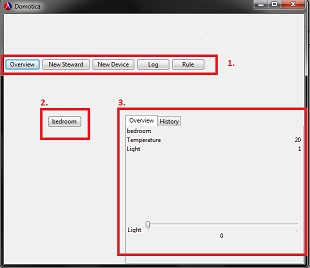
\includegraphics{../screenshot/main-menu.jpg}
			\end{center}
			\caption{Het hoofdscherm.}
		\end{figure}
	
	\begin{enumerate}
		\item Hier is het mogelijk om in de verschillende onderdelen van de applicatie te navigeren.
		\item Een lijst van de bestaande stewards.
		\item Een overzicht van de geselecteerde steward. Die bestaat uit een geschiedenis van de elementen (temperatuur...) over de tijd, de huidige waarde van de elementen en de mogelijkheid om 	die aan te passen.
	\end{enumerate}
	
		\subsection{Device Toevoegen}
		\label{add-device}
	In dit menu is het mogelijk om een nieuw type device toevoegen. Een device bestaat uit een aantal sensoren en actuatoren die gekozen kunnen worden uit de lijst of toegelaten sensoren en activatoren. Een steward kan alleen bestaande types devices beheersen, deze moeten dus op voorrand in dit menu worden toegevoegd.
	
		\newpage
		\begin{figure}
			\begin{center}
				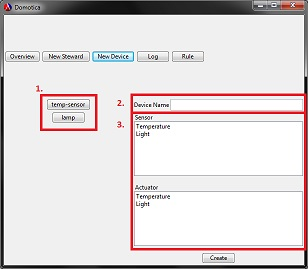
\includegraphics{../screenshot/new-device.jpg}
			\end{center}
			\caption{Voeg een nieuw device toe.}
		\end{figure}
	
		\begin{enumerate}
			\item Een lijst van de bestaande type devices.
			\item Vul hier de naam van het nieuwe device in.
			\item Kies tussen de toegelaten sensoren en activatoren.
		\end{enumerate}
	
		\subsection{Steward Toevoegen}
		\label{add-steward}
	In dit menu is het mogelijk om nieuwe stewards toe te voegen aan het domotica-programma (Figure \ref{new-steward}). Een steward beheerst een aantal devices, de serial-nummers van deze devices worden gevraagd zodat de steward ermee kan communiceren (Figure \ref{new-steward-confirmation}).
	
		\newpage
		\begin{figure}
			\begin{center}
				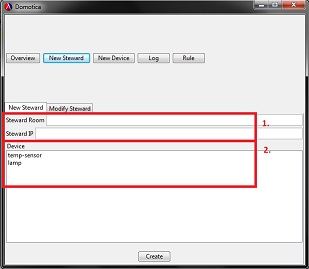
\includegraphics{../screenshot/new-steward.jpg}
			\end{center}
			\caption{Voeg een nieuwe steward toe.}
			\label{new-steward}
		\end{figure}
	
		\begin{enumerate}
			\item Voeg de naam van de steward en zijn IP adres toe.
			\item Voeg devices toe die in deze lijst inbegrepen zijn.
		\end{enumerate}
	
		\begin{figure}
			\begin{center}
				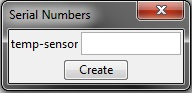
\includegraphics{../screenshot/new-steward-confirmation.jpg}
			\end{center}
			\caption{Vul de serial-numbers van de gekozen devices}
			\label{new-steward-confirmation}
		\end{figure}

		\subsection{Rule Toevoegen}
		\label{add-rule}
		De gebruiker heeft de mogelijkgheid om rules toe te voegen aan het domotica-systeem. Een rule is een instructie die op een bepaald tijdstip automatisch uitgevoerd wordt.
		
		\newpage
		\begin{figure}
			\begin{center}
				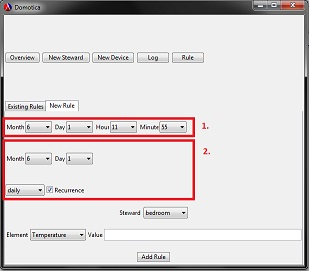
\includegraphics{../screenshot/new-rule.jpg}
			\end{center}
			\caption{Voeg een nieuwe rule toe.}
			\label{new-rule}
		\end{figure}
	
		\begin{enumerate}
			\item Het moment wanneer de rule uitgevoerd zal worden.
			\item Als 'recurrence' geselecteerd is, bestaat er de mogelijkheid om de rule dagelijks of wekelijks te herhalen tot een einddatum.
		\end{enumerate}
		
\end{document}